\documentclass[11pt]{article}
\usepackage[a4paper, top=3cm, bottom=3cm]{geometry}

\usepackage[dutch]{babel}
\selectlanguage{dutch}

\usepackage{color}
\definecolor{gray75}{gray}{0.75}

\usepackage{framed}

\usepackage{graphicx}
\usepackage{tikz}

\usepackage{subcaption}
\usepackage{wrapfig}

\usepackage{amsmath}

\usepackage[colorlinks=true,linkcolor=black]{hyperref}

\usepackage[T1]{fontenc}
\usepackage{titlesec}

\newcommand{\hsp}{\hspace{15pt}}

\titleformat{\chapter}[hang]{\Huge\bfseries}{\thechapter\hsp\textcolor{gray75}{|}\hsp}{0pt}{\Huge\bfseries}
\titlespacing{\chapter}{0pt}{-3.5ex plus 1ex minus .2ex}{2.3em plus .2ex}

\newlength{\leftbarwidth}
\setlength{\leftbarwidth}{3pt}
\newlength{\leftbarsep}
\setlength{\leftbarsep}{10pt}

\newcommand*{\leftbarcolorcmd}{\color{leftbarcolor}}% as a command to be more flexible
\colorlet{leftbarcolor}{black}

\renewenvironment{leftbar}{%
    \def\FrameCommand{{\leftbarcolorcmd{\vrule width \leftbarwidth\relax\hspace {\leftbarsep}}}}%
    \MakeFramed {\advance \hsize -\width \FrameRestore }}{\endMakeFramed}

\usepackage{pdfpages}

\begin{document}

\begin{titlepage}
\begin{center}
{\huge\bfseries A New Field-Effect Transistor with Selectively Doped $GaAs/n-Al_{x}Ga_{1-x}As$ Heterojunction}
\\ \bigskip
{\Large Discussie \& kwalitatieve analyse}
\end{center}
\vfill
\begin{flushleft}
\setlength{\leftbarwidth}{1pt}
\colorlet{leftbarcolor}{gray75}
\begin{leftbar}
Jelle Verstraaten, 500236946 \\
\texttt{jelle@benext.nl} \\
E-technology \\
Halfgeleiders \\
Erik Steuten\\
{\small \today} \\
\end{leftbar}
\end{flushleft}
\end{titlepage}

\newpage
\tableofcontents
\newpage

\section{Inleiding}
%In dit hoofdstuk wordt ingegaan op de de schrijvers van het artikel, het onderzoeklaboratorium waar zij werkten en het artikel in het algemeen.

Het artikel dat behandeld wordt, ``A New Field-Effect Transistor with Selectively Doped $GaAs/n-Al_{x}Ga_{1-x}As$ Heterojunction'', is geschreven door Takashi Mimura, Satoshi Hiyamizu, Toshio Fuji en Kazuo Nanbu in 1980. Het artikel is gepubliceerd in het Japanese Journal of Applied Physics (JJAP), een blad dat alleen artikelen accepteert die gepeer-reviewed zijn. Het artikel borduurt voort een artikel van Dingle et al (Bell Laboratories): ``Electron mobilities in modulation-doped semiconductor heterojunction superlattices''.

Het artikel is gepubliceerd in opdracht van Fujitsu Laboratories Ltd. Fujitsu was ge\"interesseerd in het vercommercializeren van de ontdekking die gedaan is door Dingle et al., namelijk dat het mogelijk was om hogere elektron-mobiliteit te behalen door een GaAs/AlGaAs heterojunction te gebruiken. %Nadat Dingle zijn onderzoek had gepubliceerd ontstond er namelijk een ware race om de eerste te zijn die deze technologie werkend te krijgen.

Er is een patent van Daniel Delagebeaudeuf en Trong L Nuyen: ``Field effect transistor with a high cut-off frequency''. Dit patent borduurt voort op het werk van Mimura et al. en Dingle et al. en bevestigt de bevindingen van beide. Delagebeaudeuf en Nuyen waren beide werkzaam bij Thomson-CSF. Dit lab was uiteindelijk in staat een betere variant van de transistor te fabriceren, die daarna patenteerd is.

De abstract is duidelijk en geeft meteen aan waarom dit nieuwe type FET interessant is. De reden is dat deze FET veel hogere frequenties (tot 3x) aankan dan de huidige ontwerpen. 

In de inleiding wordt duidelijk gemaakt dat dit artikel voortborduurt op het artikel van Dingle et al. In dit artikel wordt een nieuw fenomeen gerapporteerd, namelijk de hogere mobiliteit van elektronen in GaAs/AlGaAs heterojunction. In het artikel wat behandeld wordt, wordt verder gegaan met deze ontdekking en wordt gekeken hoe deze hogere mobiliteit gebruikt kan worden in nieuwe halfgeleidercomponenten. Ook worden er pogingen gedaan om de karakteristieken van deze nieuwe heterojunctions te achterhalen. De inleiding geeft een goed beeld van de context waarin het artikel geschreven is.

\section{Discussie}
De hoofdvraag van dit artikel is: ``Kan de hogere elektronmobiliteit van een heterojunction gebruikt worden voor het fabriceren van een snellere transistor?''. Deze hoofdvraag wordt experimenteel bevestigd door het cree\"eren van onder andere transistoren, diodes en hall-bruggen en het testen hiervan.

Om deze vraag te beantwoorden is gekozen voor een kwantitatieve onderzoeksmethode. Om te kijken of het mogelijk was om transistoren te maken zijn deze eerst gefabriceerd, hierna zijn deze getest. Hierbij werd specifiek gekeken of deze dezelfde verschijnselen vertonen als die uit het voorgaande onderzoek van Dingle et al. Daarna zijn de karakteristieken van deze nieuwe transistor vergeleken met een andere type transistor dat hetzelfde doel heeft en dezelfde fysieke opbouw en afmetingen.

De resultaten van de testen bevestigen de voorgaande bevindingen van Dingle et al. en wijzen erop dat er een 2-dimensionaal elektrongas ontstaat. Ook wordt aangetoond dat het mogelijk is om het elektrongas te moduleren door het drain-voltage $V_{DS}$ op de transistor te vari\"eren. Deze resultaten zijn belangrijk omdat hiermee de onderzoeksvraag beantwoord kan worden. Ook kan uit deze resultaten afgeleid worden dat dit nieuwe transistorontwerp, op hoge frequenties, inderdaad beter werkt dan andere ontwerpen.

\newpage

\section{Resultaten}
In het artikel worden verschillende testen gedaan om te controlleren of de transistor werkt zoals wordt verwacht. In de figuren 1a en 1b wordt toegelicht hoe de heterojunction die getest wordt is opgebouwd. Hierbij wordt gekeken naar zowel de fysieke structuur (figuur 1a) als naar de bandenstructuur (figuur 1b).
In figuur 2 wordt gekeken of het effect van het 2-dimensionaal elektrongas gereproduceerd kan worden en hoe sterk dat is. Daarna wordt gekeken naar hoe goed de geleiding is van de nieuwe transistor. Dit gebeurt in figuur 3.

De resultaten worden in het artikel duidelijk en helder gepresenteerd. Alle metingen worden duidelijk toegelicht en deze zijn ook allemaal reproduceerbaar doordat alle schalen en gekozen meetbereiken genoemd worden. Ook hebben de onderzoekers geprobeerd een zo goed mogelijke vergelijking te vinden voor de nieuwe transistor.

\begin{figure}[h]
  \centering
  \begin{subfigure}[b]{0.45\textwidth}
    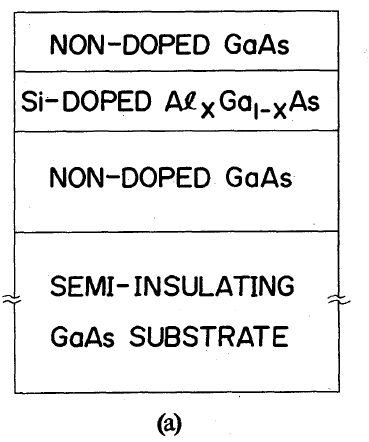
\includegraphics[width=\textwidth]{physical_structure.png}
    \caption{De fysieke opbouw van de getestte heterojunction}
    \label{fig:phsyical_structure}
  \end{subfigure}
  ~
  \begin{subfigure}[b]{0.45\textwidth}
    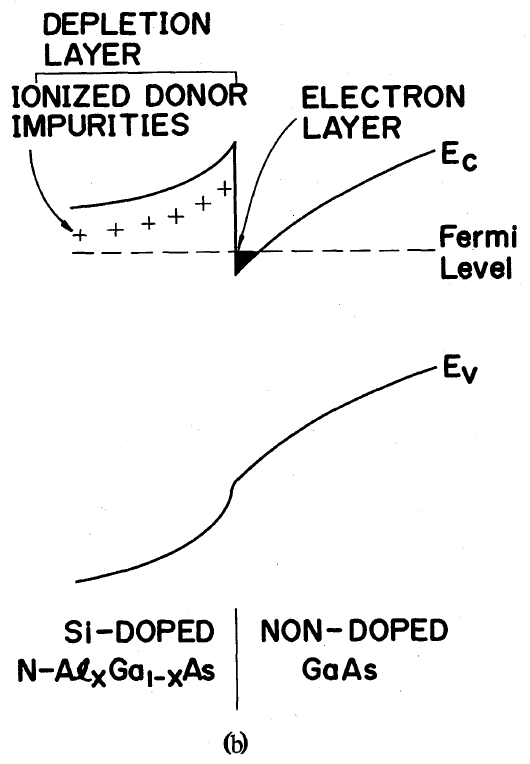
\includegraphics[width=\textwidth]{bandenergy_structure.png}
    \caption{Opbouw van de bandenstructuur van de getestte heterojunction}
    \label{fig:band_structure}
  \end{subfigure}
\end{figure}

\subsection{Figuur 1a}
In figuur 1a wordt de fysieke opbouw van de getestte heterojunction schematisch weergegeven. In de tekst wordt toegelicht wat de afmetingen van de lagen zijn en hoe sterk deze gedoteerd zijn.

Ook wordt aangegeven dat deze structuur gecree\"erd is met behulp van MBE (molecular beam epitaxy). Dit is een manier om hoogkristalleine lagen aan te brengen op een substraat. De aanwezigheid van deze gegevens is nuttig en noodzakelijk, aangezien het zonder deze niet mogelijk is om het onderzoek te reproduceren.

\subsection{Figuur 1b}
In figuur 1b wordt gekeken naar de elektrische bandenstructuur van de heterojunction. In dit diagram wordt ge\"illustreerd hoe de bandenstructuur ervoor zorgt dat er een 2-dimensionaal elektrongas ontstaat. 

Er wordt in het artikel weinig ingegaan op waarom er sprake is van ``electron-confinement'' en waarom de elektronen van de donor naar de GaAs-laag migreren. Dit wordt kort aangestipt in de introductie van het artikel. Hier wordt verwezen naar de metingen van Dingle et al. en uitgelegt dat de elektronen naar de GaAs-laag migreren omdat deze een hogere ``elektronenaffiniteit'' heeft. Dit houdt in de elektronen makkelijker kunnen bewegen in de GaAs-laag, omdat ze hier niet afgeremt worden door de donoronzuiverheden.

\subsection{Figuur 2}
In figuur 2 wordt de ``apparent carrier profile'' weergegeven zoals gemeten op 77K. De ``apparent carrier profile'' geeft aan wat de lading (elektronen)dichtheid is op een bepaalde diepte van het substraat.

Dit dichtheidsprofiel is gemeten met behulp van een ``differential capacitance feedback profiler''. Door een voltage over de heterojunction te zetten en dan capaciteit te bepalen kan volgens Kro\"emer et al. bepaald worden hoeveel ladingsdragers er aanwezig zijn op een bepaalde diepte.

De duidelijk waarneembare piek kan volgens de auteurs duiden op de aanwezigheid van een 2-dimensionaal elektrongas.

\begin{figure}[h]
  \begin{center}
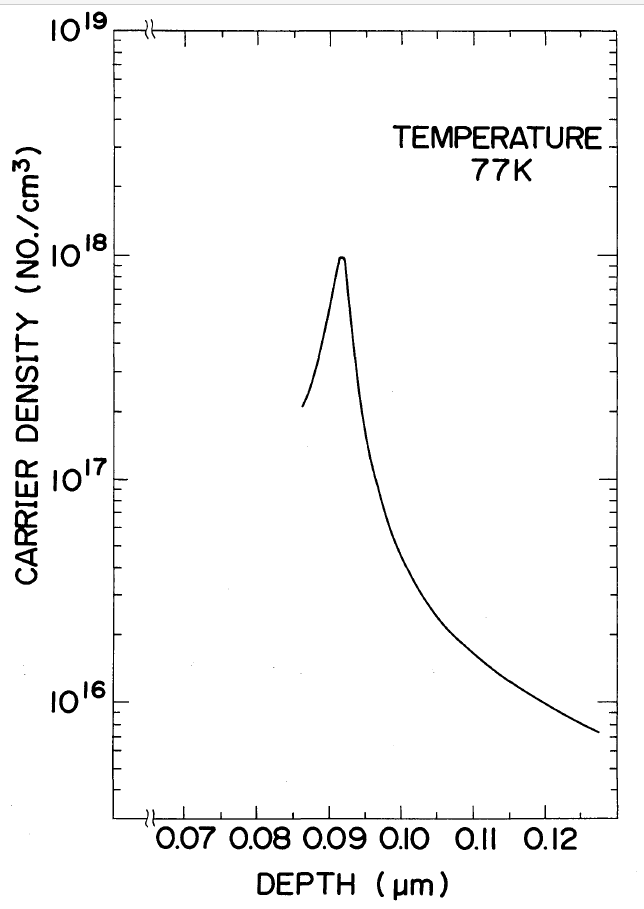
\includegraphics[width=0.5\textwidth]{carrier_profile_depth.png}
\caption{Dichtheid van ladingdragers als functie van de doorsnee van de heterojunction. Er is een duidelijk waarneembare piek die kan mogelijk ontstaat door de aanwezigheid van een 2-dimensionaal elektrongas}
\label{fig:carrierprofile}
  \end{center}
\end{figure}

\subsection{Figuur 3}
In figuur 3 wordt het stroom-voltage-karakteristiek van het nieuwe type transistor vergeleken met een bestaand type transistor op 300K en op 77K. Er wordt duidelijk toegelicht wat de afmetingen van de heterojunction zijn en op welke voltage en amperage er gemeten is.

Uit de grafieken is duidelijk af te leiden dat het nieuwe type transistor (figuur 3a) voornamelijk op lage temperaturen een veel betere geleiding heeft. Bij kamertemperatuur is effect wel duidelijk meetbaar, maar lang niet zo sterk. Dit is voornamelijk om dat de elektronmobiliteit toeneemt op lage temperaturen. 

Het gaat hier volgens het artikel om 30\% meer geleiding bij 300K en tot wel 6x  meer geleiding bij 77K. Dit is te zien aan de grotere spreiding tussen de lijnen in figuur 3a. Deze lijnen drukken de waardes uit in geleiding ($G_m$) of wel  $1/R$. In het artikel wordt daarna aangetoond dat een beter geleiding direct te vertalen is naar een hogere bandbreedte voor de transistor.

De onderzoekers hebben geprobeerd om de vergelijkingstransistor zoveel mogelijk hetzelfde te krijgen als het nieuwe type. De nieuwe HEMT-transistor heeft, zoals te zien in figuur 2, rond de heterojunction een ladingdichtheid van minimaal $\pm2*10^{17}/cm^3$. De MESFET waarmee vergeleken wordt is daarom zo gedoteerd dat deze een ladingdichtheid van $1.0 * 10^{17}/cm^3$ heeft. Ook is geprobeerd om de gate-, source- en drain-geometrie hetzelfde te houden zodat deze dezelfde capaciteit hebben.

\begin{figure}[h]
  \begin{center}
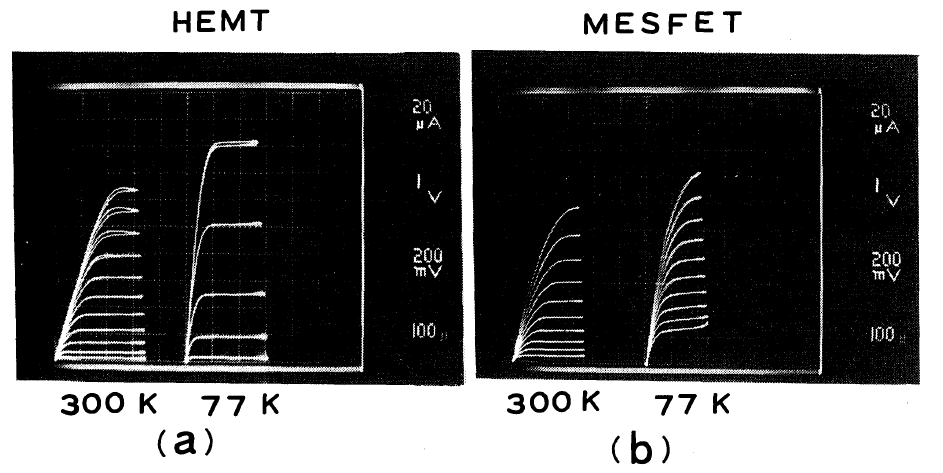
\includegraphics[width=\textwidth]{CV-characteristics.png}
\caption{Vergelijking van de stroom-voltage-karakteristiek van een HEMT-FET(a) en een MESFET(b)}
\label{fig:cv_karakteristieken}
  \end{center}
\end{figure}

\newpage

\section{Experimenten}
Voor het testen van het nieuwe type transistor zijn 2 testen gedaan: capaciteit-voltage-profilering en stroom-voltage-karakteristiek bepaling.

\subsection{Capaciteit-voltage-profilering}
Capaciteit-voltage-profilering of CV-profilering is een techniek die gebruikt wordt om de interne structuur van een heterojunction te bepalen. Door een spanning over de heterojunction te zetten wordt een ``depletion-region'' gecree\"erd. Deze bevat geen elektronen of gaten meer, maar heeft nog wel een intrinsieke lading vanwege de aanwezig donoratomen. Deze intrinsieke lading cree\"ert een capaciteit die meetbaar is. Door de spanning over de heterojunction te varie\"eren kan de ``depletion-region'' groter of kleiner gemaakt worden, waardoor gekeken kan worden naar verschillende delen van de heterojunction.

De resultaten van deze test zijn te vinden in figuur 2 van het artikel. In dit grafiek is de gemeten capaciteit omgezet naar een ladingsdichtheid.

\subsection{Stroom-voltage-karakteristiekbepaling}
De stroom-voltage-karakteristiek of IV-curve is een manier waarop de parameters van een transistor bepaald kunnen worden. Door een vaste stroom aan te bieden op de gate (of base) van een transistor en de spanning over de source-drain of (collector-emitter) te vari\"eren kan bepaald worden wanneer de transistor volledig ``aan'' is en hoe lineair de versterking is van de transistor. Ook kan de zogenaamde ``small-signal applification'' of $H_{fe}$ bepaald worden.

De resultaten van deze test zijn te vinden in figuur 3. In dit grafiek wordt ook de vergelijking gemaakt tussen de nieuwe transistor een een vergelijkbaar, al bekend, ontwerp.

\section{Referenties}
Het artikel gebruikt de ACS of ``American Chemical Society''-referentiestijl. Deze stijl volgt het volgende format: Achternaam, Initialen.; Achternaam, Initialen. tijdschrift. jaar, Volume, paginas. 

Alle referenties in het artikel komen slechts 1 keer voor, maar het belangerijkste artikel is het eerst vermeldde artikel: ``Electron mobilities in modulation-doped semiconductor heterojunction superlattices''. De wetenschappers hebben namelijk geprobeerd om de nieuwe bevindingen uit dit artikel te reproduceren en toe te passen en in nieuw type transistor.

\appendix

\addcontentsline{toc}{section}{A New Field-Effect Transistor with Selectively Doped $GaAs/n-Al_{x}Ga_{1-x}As$ Heterojunction}
\includepdf[pages=2-]{1347-4065_19_5_L225.pdf}

\addcontentsline{toc}{section}{Electron mobilities in modulation-doped semiconductor heterojunction superlattices}
\includepdf[pages=2-]{190457.pdf}

\end{document}

%Inleverdatum: 2015-06-22
%Herkansing: 2015-08-31
